\subsection{Performance of the Filter}
The performance of the Kalman filter can be tested through simulation, where the estimation is compared to the real value given by the simulation.

The measurements are simulated by adding noise, whose variances are the ones coming from the real sensors as seen in \autoref{app:IMUVariances}, to the real values.

 The filter is able to remove some noise present in the measurements as seen in the heading estimation in \autoref{fig:sim_yaw}.
\begin{figure}[H]
    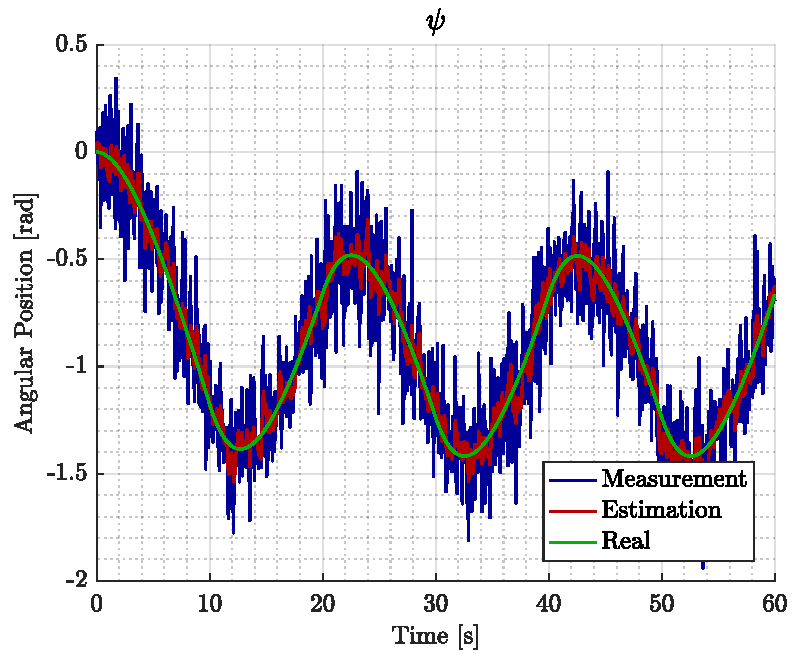
\includegraphics[width=0.5\textwidth]{figures/sim_yaw}
    \caption{Result of the estimation of the heading, compared to the real value in the simulation and the measurements.}
    \label{fig:sim_yaw}
\end{figure}
%
The estimation of the angular velocity and acceleration around $z_\mathrm{b}$ can be seen in \autoref{fig:sim_yawdot} and \ref{fig:sim_yawddot}, respectively.
%
\begin{figure}[H]
    \captionbox 
    {   
        Result of the estimation of the angular velocity around $z_\mathrm{b}$, compared to the real value in the simulation and the measurements.
        \label{fig:sim_yawdot}
    }                                                                 
    {                                                                  
        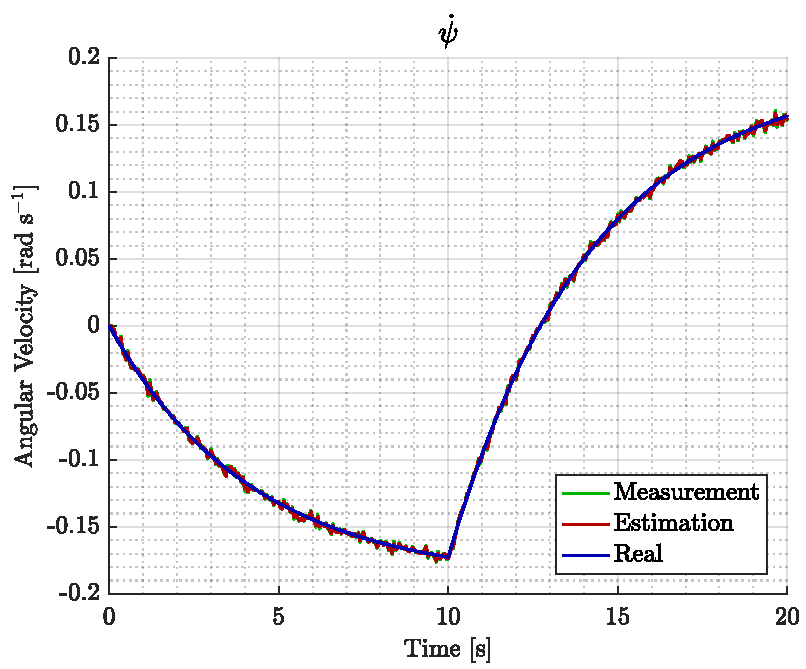
\includegraphics[width=.45\textwidth]{figures/sim_yawdot}         
    }                                                                    
    \hspace{5pt}                                                          
    \captionbox  
    {      
        Estimation of the angular acceleration around $z_\mathrm{b}$, compared to the real value.
        \label{fig:sim_yawddot}
    }                                                                          
    {
        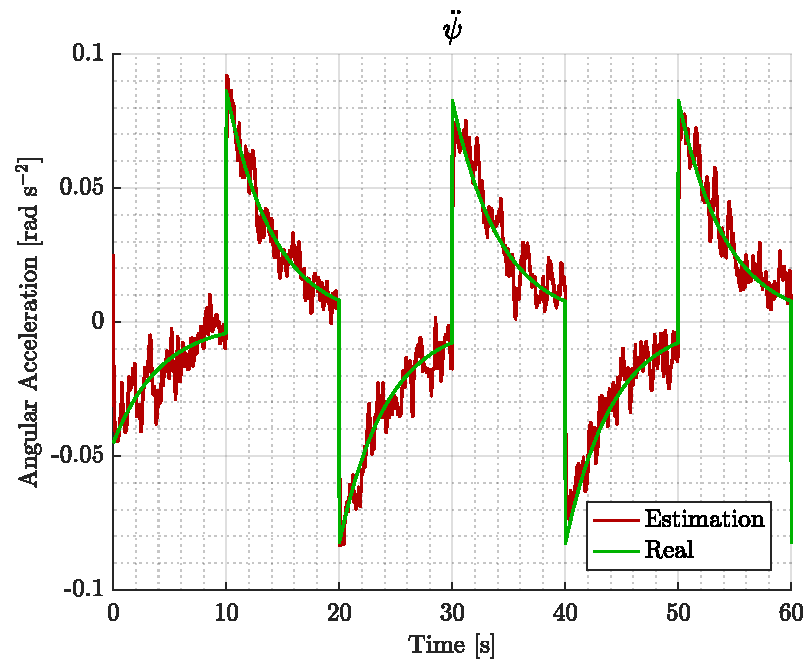
\includegraphics[width=.45\textwidth]{figures/sim_yawddot}
    }
\end{figure}
%
It is noticeable that there is no direct measurement of the angular acceleration, and the estimation is able to follows the real value from the simulation.

\begin{figure}[H]
    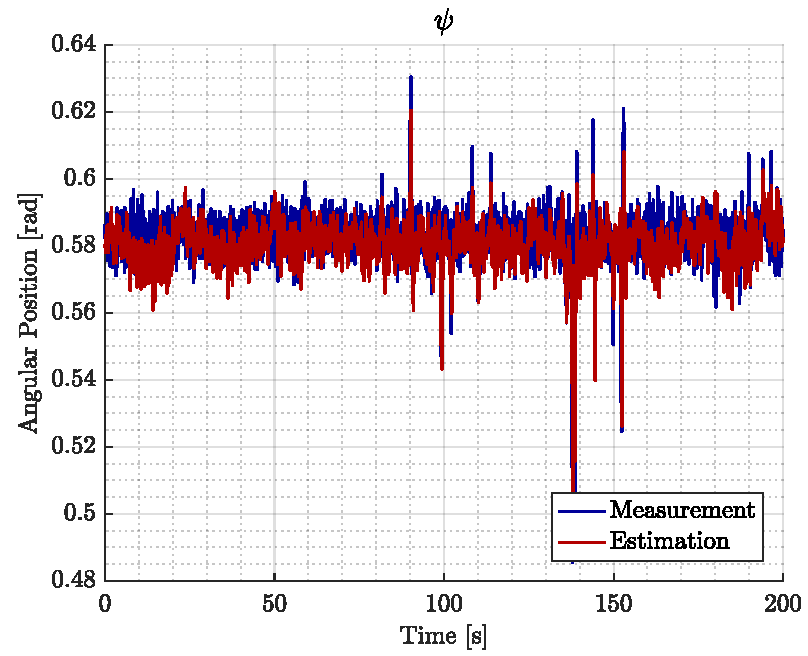
\includegraphics[width=0.5\textwidth]{figures/real_yaw}
    \caption{}
    \label{fig:real_yaw}
\end{figure}

\begin{figure}[H]
    \captionbox 
    {   
        Result of the estimation of the angular velocity around $z_\mathrm{b}$, compared to the measurements.
        \label{fig:real_yawdot}
    }                                                                 
    {                                                                  
        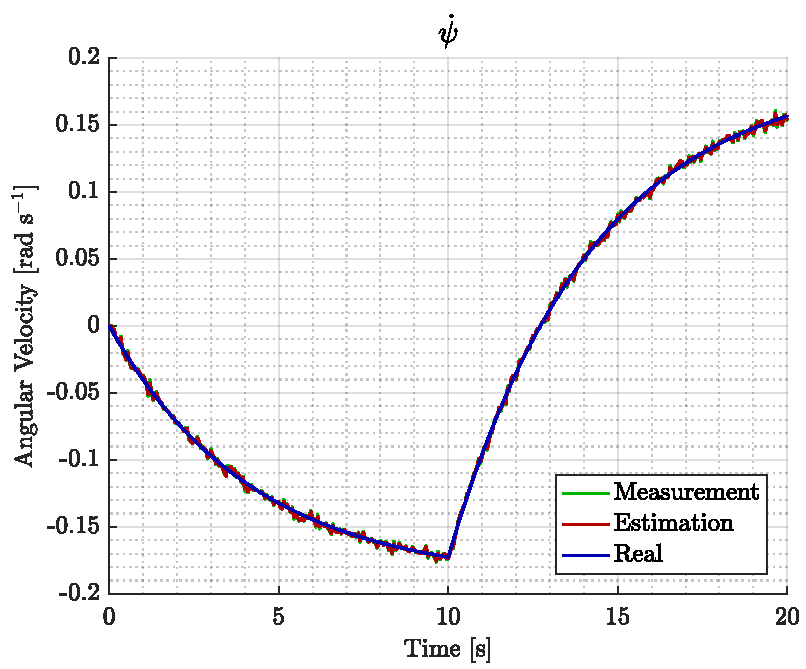
\includegraphics[width=.45\textwidth]{figures/sim_yawdot}         
    }                                                                    
    \hspace{5pt}                                                          
    \captionbox  
    {      
        Estimation of the angular acceleration around $z_\mathrm{b}$.
        \label{fig:real_yawddot}
    }                                                                          
    {
        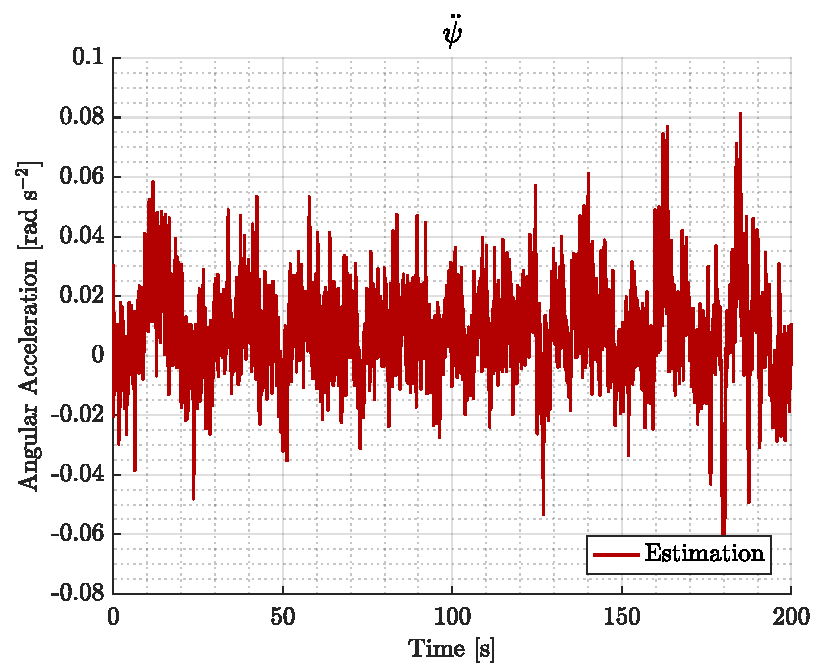
\includegraphics[width=.45\textwidth]{figures/real_yawddot}
    }
\end{figure}

\cite{MSalari}